\documentclass[a4paper,11pt]{article}
\author{Quelli della B1}
\usepackage[utf8]{inputenc}
\usepackage[italian]{babel}
\usepackage{graphicx}
\usepackage[colorlinks=true,linkcolor=blue]{hyperref}
\usepackage{hyperref}
\usepackage{nameref} 
\graphicspath{{./images/}}

\def\code#1{\texttt{#1}}
\def\sec#1{\section{#1}\label{#1}} 
\def\sub#1{\subsection{#1}\label{#1}} 
\def\subsub#1{\subsubsection{#1}\label{#1}} 
\def\vedi#1{\nameref{#1}} 

\title{Networking}

\begin{document}

\maketitle
\newpage
\tableofcontents
\newpage

\sec{Introduzione}
%Gioara 
\sub{Il modello di riferimento ISO/OSI}
Il modello Open Systems Interconnection (abbreviato in modello ISO/OSI) è stato progettato dall’International Organization for Standardization (ISO) come modello di riferimento per consentire una comunicazione aperta tra diversi sistemi tecnici. Questo punto diventa più chiaro, se si pensa alle origini di Internet: alla fine degli anni ’70 i leader del settore nelle tecnologie di rete si ritrovarono di fronte al problema che le architetture di rete proprietarie si potevano collegare solo tramite dispositivi propri, infatti nessun produttore aveva pensato di costruire componenti hardware o software compatibili con le specificazioni di altri fornitori. Ma un progetto come quello di Internet presuppone alcuni standard per poter rendere possibile una comunicazione comune.
Il modello lSO/OSI è nato dal tentativo di creare uno standard di questo tipo e offre una base per gli standard di comunicazione, indipendentemente dai fornitori. In base a questo modello, il complesso processo della comunicazione di rete si divide in sette strati, i livelli (in inglese layer). Si parla perciò anche di una comunicazione per livelli. All’interno della comunicazione tra due sistemi devono essere svolti degli specifici compiti su ogni singolo livello, tra questi rientrano ad esempio il controllo della comunicazione, l’indirizzamento del sistema target o la conversione dei pacchetti in segnali fisici. Ma questo funziona solo se tutti i sistemi coinvolti nella comunicazione si attengono a regole precise, stabilite nei protocolli, che si applicano ai singoli livelli o si possono utilizzare su ciascuno di questi (multilivello).
\\Il modello di riferimento ISO/OSI non è però uno standard di rete concreto, ma descrive in forma astratta quali procedimenti devono essere regolati per far funzionare la comunicazione in una rete.  
\subsub{I livelli}
La comunicazione tra due computer può apparire banale agli utenti, ma in realtà durante la trasmissione di dati in una rete devono essere compiuti numerosi compiti e soddisfatte diverse richieste nell’ambito dell’attendibilità, della sicurezza e dell’integrità. Per questo si è deciso di dividere la comunicazione di rete in livelli. Ad ogni livello, strutturato gerarchicamente, sono assegnate delle funzioni specifiche (quindi uno standard copre generalmente solo una parte del modello): ogni livello accede tramite un’interfaccia a quello inferiore e mette a disposizione il servizio del livello superiore.
\\Questo principio ha due vantaggi decisivi:
\begin{itemize}
	\item I compiti e le richieste che devono essere compiuti e soddisfatti all’interno di un livello sono definiti chiaramente. Per ogni livello possono essere sviluppati degli standard indipendenti gli uni dagli altri.
	\item La chiara divisione tra i singoli livelli fa sì che le modifiche ad uno standard non abbiano alcun effetto sui processi che si svolgono su un altro livello. Introdurre nuovi standard risulta così più semplice.
\end{itemize}
I sette livelli del modello ISO/OSI si dividono in due gruppi in base ai compiti che svolgono: orientati all’applicazione e orientati al trasporto. I processi che si svolgono sui singoli livelli si possono spiegare prendendo ad esempio la trasmissione e-mail da un dispositivo ad un mail server.

\sub{Internet protocol suite (TCP/IP)}

\newpage

\sec{Livello Fisico}
Nonostante l'amministratore di rete non abbia la possibilità di influirvi direttamente, è importante descrivere lo strato fisico poiché esso influenza significativamente le prestazioni della rete.

\subsection{Terminologia}
\subsub{Informazione} 
L'informazione è una grandezza misurabile in bit. In particolare, \[Q=log_{2}m\] dove $Q$ è il numero di bit necessari per rappresentare l'informazione relativa ad $m$ possibili stati. 

\subsub{Codice}
Al fine di rappresentare l'informazione in maniera tale da renderne più semplice la gestione, un codice associa sequenze di bit a caratteri. I codici che godono della più ampia diffusione sono:
\begin{itemize}
\item ASCII (American Standard Code for Information Interchange, 7 bit estesi a 1 byte)
\item BCD (Binary-Coded Decimal)
\item AIKEN 
\item Gray
\item EBCDIC (Extended Binary Coded Decimal Code, 8 bit), in uso presso le banche
\end{itemize}

\subsubsection{Segnale}
Si dice \textit{segnale} una grandezza fisica variabile nel tempo corrispondente un'informazione. Un segnale \textbf{analogico} varia in modo continuo nel tempo ed ha infiniti livelli di intensità; un segnale \textbf{digitale} varia invece in modo discreto e ha solo due livelli di intensità. Ogni tipo di dato può essere rappresentato in entrambe le maniere e può essere convertito da analogico a digitale e viceversa.
\\\\Fra i segnali analogici assumono particolare rilevanza i \textbf{segnali sinusoidali}, ossia segnali che variano nel tempo secondo una legge del tipo \[u=Usen(\omega t+\Phi )\] dove 
\begin{itemize}
\item $u$ è l'ampiezza istantanea
\item $U$ è l'ampiezza massima
\item $\omega $ è la velocità angolare 
va spiegato meglio
\item $\Phi $ è lo sfasamento rispetto all'origine
\item l'intervallo di tempo impiegato dall'onda per tornare allo stesso livello d'intensità è detto \textit{periodo}.
\item $1/t=f$ è detta \textit{frequenza} (misurabile in Hz)\\\\
\end{itemize}
La curva in figura rappresenta istante per istante il valore del seno dell'angolo descritto da un segmento che ruota con un estremo vincolato all'origine degli assi cartesiani, in senso antiorario, con velocità angolare $\omega $. Di conseguenza, la frequenza $f$ è il numero di volte che il segmento effettua un giro completo.
\begin{figure}
\centering
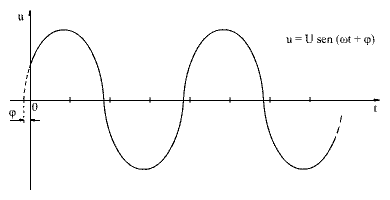
\includegraphics[scale=0.5]{segnali_sin.png}
\caption{Rappresentazione grafica di un segnale sinusoidale}\label{fig. 1}
\end{figure}

\subsubsection{Lunghezza d'onda}
In un segnale sinusoidale, la distanza tra due massimi relativi è detta \textit{lunghezza d'onda} $\lambda =c/f$ (dove $c$ è la velocità di propagazione del segnale).

\subsub{Spettro}
Lo spettro è l'insieme delle frequenze che compongono un segnale. Questa affermazione, non necessariamente di immediata comprensione, diventa subito chiara se si tiene presente il \textbf{teorema di Fourier}, il quale afferma che un segnale può essere rappresentato come somma di sinusoidi (potenzialmente infinite) con caratteristiche differenti.

\subsub{Ampiezza di banda}
L'ampiezza di banda è costituita dall'insieme di frequenze dello spettro \textit{effettivamente utilizzate} e corrisponde alla massima velocità teorica della rete. Si parla di \textit{banda larga} nel caso in cui l'ampiezza di banda sia sensibilmente superiore a quella utilizzata correntemente per le comunicazioni telefoniche.

\subsection{Qualità delle trasmissioni}
Come già accennato in precedenza, é lo strato fisico che determina in larga parte la qualità delle comunicazioni, valutabile in base a prestazioni e affidabilità. 
\\Vi sono numerosi strumenti software per valutare la qualità di una rete, quali:
\begin{itemize}
\item il comando Unix \code{ping}, che indica se un host remoto possa essere raggiunto e riporta statistiche sui pacchetti persi
\item il comando Unix \code{traceroute} o \code{tracepath}, che indica i dispositivi attraversati per raggiungere una data destinazione
\item applicazioni web quali ad esempio \url{speedtest.net} e \href{<https://www.misurainternet.it/>}{Ne.Me.Sys}, quest'ultimo sviluppato da AGCOM, i cui risultati possono essere utilizzati come elemento probatorio nel caso in cui l’utente voglia esercitare il diritto di reclamo e recesso rispetto a promesse contrattuali di velocità di accesso ad Internet non mantenute dall‘operatore.
\end{itemize}

\subsub{Criteri di valutazione in base alle prestazioni}
\begin{itemize}
\item \textbf{ritardo}: tempo necessario per il transito dei dati
\item \textbf{tempo di risposta}: tempo che intercorre tra il momento in cui viene effettuata una richiesta e il momento in cui si ottiene una risposta
\item \textbf{throughput}: quantità di dati spedita nell'unità di tempo; rappresenta l'effettiva velocità della rete
\item \textbf{latenza}: tempo necessario perché un messaggio giunga a destinazione; per il suo calcolo si tiene conto di:
\begin{itemize}
\item \textbf{tempo di propagazione}: tempo di transito sulla rete per arrivare dal mittente al destinatario
\item \textbf{tempo di trasmissione}: tempo necessario per immettere i bit sulla rete, ossia $\frac{dim_{m}}{v}$, dove $dim_{m}$ è la dimensione del messaggio e $v$ la velocità trasmissiva
\item \textbf{tempo di inoltro}: tempo necessario ai nodi per consegnare il messaggio in transito, non legato al traffico ma solo ad hardware e software
\item \textbf{tempo di attesa} nelle code di rete, dipendente dal traffico
\end{itemize}
\subsubsection{Criteri di valutazione in base all'affidabilità}
\item \textbf{jitter}: variabilità del ritardo con cui i pacchetti vengono consegnari in ricezione
\item \textbf{packet loss}: pacchetti persi.

\sub{Filtri}
\end{itemize}
Un filtro è un sistema che tratta le varie componenti del segnale in modo diverso a seconda della loro frequenza.
\\E' opportuna innanzitutto una distinzione tra filtri \textit{passivi} ed \textit{attivi}: i primi sono costituiti solamente da resistenze e condensatori, mentre i secondi includono altre componenti, come i transistor e gli amplificatori. Inoltre, a seconda del comportamento, si distinguono quattro tipi di filtri:
\begin{itemize}
\item \textbf{filtro passa basso}: permette il passaggio delle frequenze al di sotto di una determinata \textit{frequenza di taglio}, definita come \[\frac{v_{out}}{v_{in}}=\frac{1}{(2)^{1/2}}\]
dove $v_{in}$ è il segnale in ingresso e $v_{out}$ il segnale in uscita.
\item \textbf{filtro passa alto}: complementare al filtro passa basso, permette il passaggio delle frequenze al di sopra della frequenza di taglio, definita come sopra
\item \textbf{filtro passa banda}: composizione di un filtro passa basso e un filtro passa alto
\item \textbf{filtro elimina banda}: complemento del filtro passa banda, blocca le frequenze comprese tra due frequenze di taglio.
\end{itemize}

\sub{Modulazione}
Sovente capita che l'informazione debba essere convertita in maniera idonea ad essere inviata nel mezzo trasmissivo adottato. Tale processo è detto \textit{modulazione} ed è reversibile: il \textit{segnale portante}, caratteristico del mezzo trasmissivo, viene modificato in uno dei suoi parametri essenziali in accordo al segnale in ingresso, contenente l'informazione da trasmettersi, che è detto \textit{segnale modulante}.
\subsub{Ad onda continua}
Si parla di modulazione ad onda continua nel momento in cui viene modulata una portante sinusoidale. Ne esistono tre tipologie:
\begin{itemize}
\item \textbf{AM} (Amplitude Modulation): l'ampiezza del segnale portante viene modulata in proporzione al segnale modulante. Per quel che riguarda la trasmissione digitale, lo 0 è associato a bassa potenza e l'1 ad alta potenza.
\item \textbf{FM} (Frequency Modulation): 
\item \textbf{PM} (Phase Modulation): 
\end{itemize}
\begin{figure}[h]
\centering
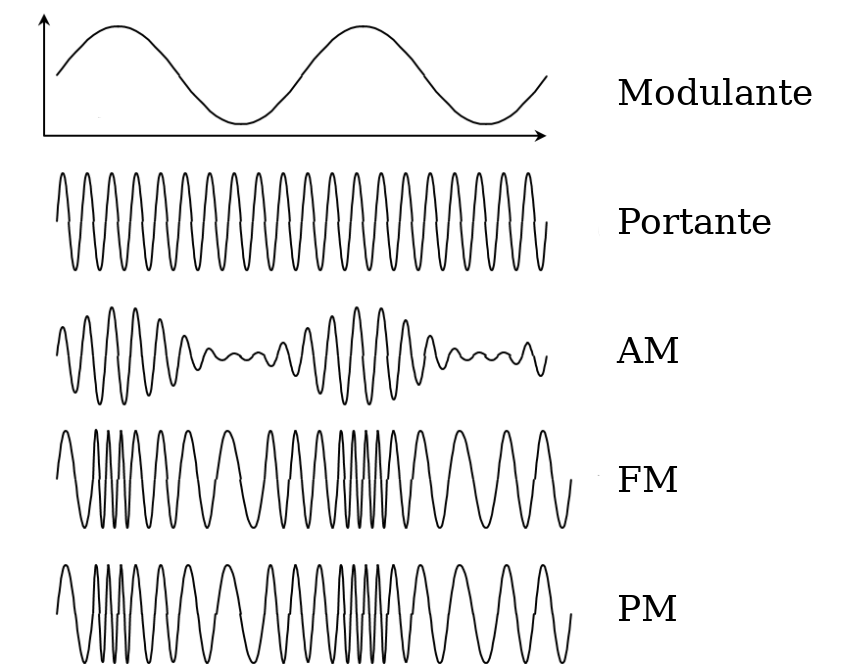
\includegraphics[scale=0.5]{am_fm_pm.png}
\caption{Confronto tra tipologie di modulazione ad onda continua}\label{fig. 2}
\end{figure}
\subsub{Impulsiva}
\subsub{Digitale}

\sub{Alterazioni del segnale}
\subsub{Attenuazione}
\subsub{Distorsione}
\subsub{Rumore}
\subsub{Interferenza}

\subsection{Limiti alla velocità di trasferimento}
\subsub{Classificazione dei canali trasmissivi}
\subsub{Teorema di Nyquist}
\subsub{Teorema di Shannon}
\subsubsection{Velocità di modulazione}
\newpage
\sec{Livello di Collegamento}
%Filippo---------------------------------------------------------------------------------------------------------------------
\sub{Tipi di trasmissione}
\subsub{Sincrona}
\subsub{Asincrona}
\subsub{Orientata al carattere}
\subsub{Orientata al bit}

\sub{Controllo degli errori}
\subsub{Ridondanza}

\sub{Protocolli primario-secondario}
\subsub{RTS-CTS}
\subsub{XON-XOF}
\subsub{ARQ}
%NB protocolli nel livello di rete?
\sub{Protocolli internet} 
\subsub{ARP} 
\subsub{RARP} 
\subsub{NDP} 
\subsub{MAC} 
 
\sub{Ethernet} 
\newpage


\sec{Livello di Rete}
%Claudio---------------------------------------------------------------------------------------------------------------------
\subsection{Terminologia}
\subsub{Rete}
Insieme di dispositivi connessi da canali di comunicazione.
\subsub{DTE}
Data Terminal Equipment: qualunque dispositivo che è la sorgente o la destinazione di una comunicazione di dati.
Un esempio è il Personal Computer (PC). 
\subsub{DCE}
Data Circuit-terminating Equipment o Data Communication Equipment: dispositivo intermedio 
tra \vedi{DTE} e il resto della rete, esegue conversioni di segnale, correzione di errori
e gestisce il clock dei dispositivi connessi. Può anche essere del \vedi{DTE}. Tipicamente è un Modem-Router.
\subsub{CPE}
Customer Premises Equipment: ISDN

\sub{Tipologie di rete}


\sub{Topologia di una rete}
\subsection{Qualità della rete}
\sub{Routing}
\subsub{Tabella di routing}
\code{netstat -nr}
\sub{Protocolli di routing}
\subsub{ICMP} 
\subsub{IGMP} 
\subsub{RIP} 
\subsub{OSPF} 

\sub{Internet Protocol (IP)} 
\newpage

\sec{Livello di trasporto}

\sub{Protocolli primario-secondario}
\subsub{RTS-CTS}
\subsub{XON-XOF}
\subsub{ARQ}
Il protocollo ARQ è di tipo \vedi{Full-Duplex}

\sub{Protocolli} 
\subsub{TCP} 
\subsub{UDP} 
\newpage

\sec{Livello delle applicazioni}
Il livello delle applicazioni racchiude tutte le applicazioni dedicate all'utente finale. 
Qui \'e dove la differenza fra protocollo e servizio si fa sempre pi\'u labile: molto spesso, la stessa parola (e.g. telnet) indica sia il protocollo, che la sua implementazione la quale, la maggior parte delle volte, \'e un comando Linux. 
\sub{Protocolli}
%Tommaso 
\subsub{Telnet e SSH} %standard odierno
Telenet nasce come protocollo di rete per sistemi Unix in grado di gestire una comunicazione standardizzata fra due \vedi{DTE}. Principalmente, Telnet, \'e sempre stato utilizzato per fornire all'utente una sessione remota del terminale dell'host. L'host ascolta sulla porta 22 e l'utente stabilisce una connessione utilizzando il public IP, nome utente e password di un Unix user dell'host. L'unico grande problema di Telnet riguarda la sicurezza: \'e un protocollo non il criptato, ovvero la password il nome utente e tutte le altre informazioni inviate, risultano completamente chiare a qualsiasi utente estraneo alla conversazione.
%Qui \'e dove il protocollo SSH 
\subsub{FTP e SCP} %standard odierno
\subsub{BGP} 
\subsub{DHCP} %Discovering ,Offering , Codice 
\subsub{DNS} 
\subsub{HTTP/HTTPS} 
\subsub{NFS}
\subsub{SNMP} %problemi sicurezza, v3, Managment Information Base (MIB), SNMP trap per gestione imprevisti, polling orientato ai trap, Structure of Management Information (SMI) 

\sub{Implementazioni}

\subsub{Telnet e SSH} %standard odierno
\subsub{FTP e SCP} %standard odierno
\subsub{DNS} 
\subsub{HTTP/HTTPS} 
\subsub{NFS}
\subsub{SNMP} %problemi sicurezza, v3, Managment Information Base (MIB), SNMP trap per gestione imprevisti, polling orientato ai trap, Structure of Management Information (SMI) 
\end{document}
